\chapter{Dark matter interpretations of Run 1 searches for invisibly decaying Higgs bosons}
\label{chap:interp}
As well as combining the results of the \ac{VBF} searches with other channels, it is also possible to interpret them as limits on other specific models. The particular models that are studied fall into two classes, \ac{EFT}s and simplified models, which are described in detail in \SectionRef{sec:DMextensions}. These studies were not carried out as part of the CMS collaboration, so it was necessary to develop and validate a framework for simulating the events resulting from these models.

%??CHECK PLOT AXIS LABEL SIZES AND THAT LEGEND TERMS ARE STANDARD OR IN TEXT

\section{Simulation Techniques and Validation}
\label{sec:dmval}
The CMS \textsc{Geant} based detector simulation is very computing intensive, so an alternative detector simulation with the \textsc{Delphes} fast reconstruction package was used. Whilst \textsc{Delphes} has been extensively validated by its authors against the CMS reconstruction~\cite{Favereau2014}, several of the variables used in the invisible Higgs boson decay searches described in this thesis were not included in this validation. Furthermore, whilst the signal process hard-scattering was simulated with Powheg in the CMS analysis, the studies described in this chapter use \textsc{MadGraph}. Both the internal CMS simulation and that described in this chapter use Pythia for parton-showering and hadronisation. Yields and kinematic distributions of events after selection criteria are applied are obtained from these simulations using an analysis framework developed and validated by the MasterCode collaboration~\cite{deVries:2015hva}.

%??start with internal sample validate against powheg plus delphes: when generated with same PU etc. found to agree to within 10% phenoplots281015.pdf
The validation of the simulations and analysis framework fall into two steps. First Powheg and pythia are used to simulate a 125 \GeV Higgs boson decaying to invisible final states, as in the internal CMS simulation. This sample of events is then processed using the \textsc{Delphes} based reconstruction and MasterCode analysis framework.
%??recreation of metsig and l1met
The resulting event yields are compared to those from the full CMS reconstruction and analysis framework and agreement to within 10\% was found.


The second step was to compare the 125 \GeV invisible Higgs boson decay sample generated with Powheg to one generated with \textsc{MadGraph} with both samples being processed using \textsc{Delphes}. This comparison was carried out at several steps of the Run 1 parked data \ac{VBF} Higgs to invisible search signal region selection, which is listed in \EquationRef{eq:parkedsigsel}. %??give starting point, say madgraph samples include vh agreement starts at ~ 15\% improves to better than 5\% as selection goes on

%??validate powheg plus delphes against mg plus delphes table from phenoplots281015.pdf
\begin{table}
  \caption{}%??explain cuts added and start point
  \label{tab:mgvspowhegdelphes}
  \begin{tabular}{lcc}
    \hline
    \hline
    Cut added & \textsc{MadGraph} + Delphes & Powheg + Delphes \\
    \hline
    Start point & 2653 & 2311 \\
    leading jet $p_{T}>50$ GeV, jet 2 $p_{T}>45$ GeV & 2056 & 1834 \\
    \METnoMU$>90$ GeV & 2000 & 1793 \\
    \Mjj$>1200$ GeV & 704 & 689 \\
    \METsig$>4$ & 539 & 519 \\
    \jetmetdphi$>2.3$ & 244 & 248 \\
    \hline
    \hline
  \end{tabular}
\end{table}

%??agreement can be seen to be good, the madgraph+delphes sim then used to generate samples at several mass points and for all the efts, met and eta for representative subsample of these shown in fig

\begin{figure}
  \subfloat[]{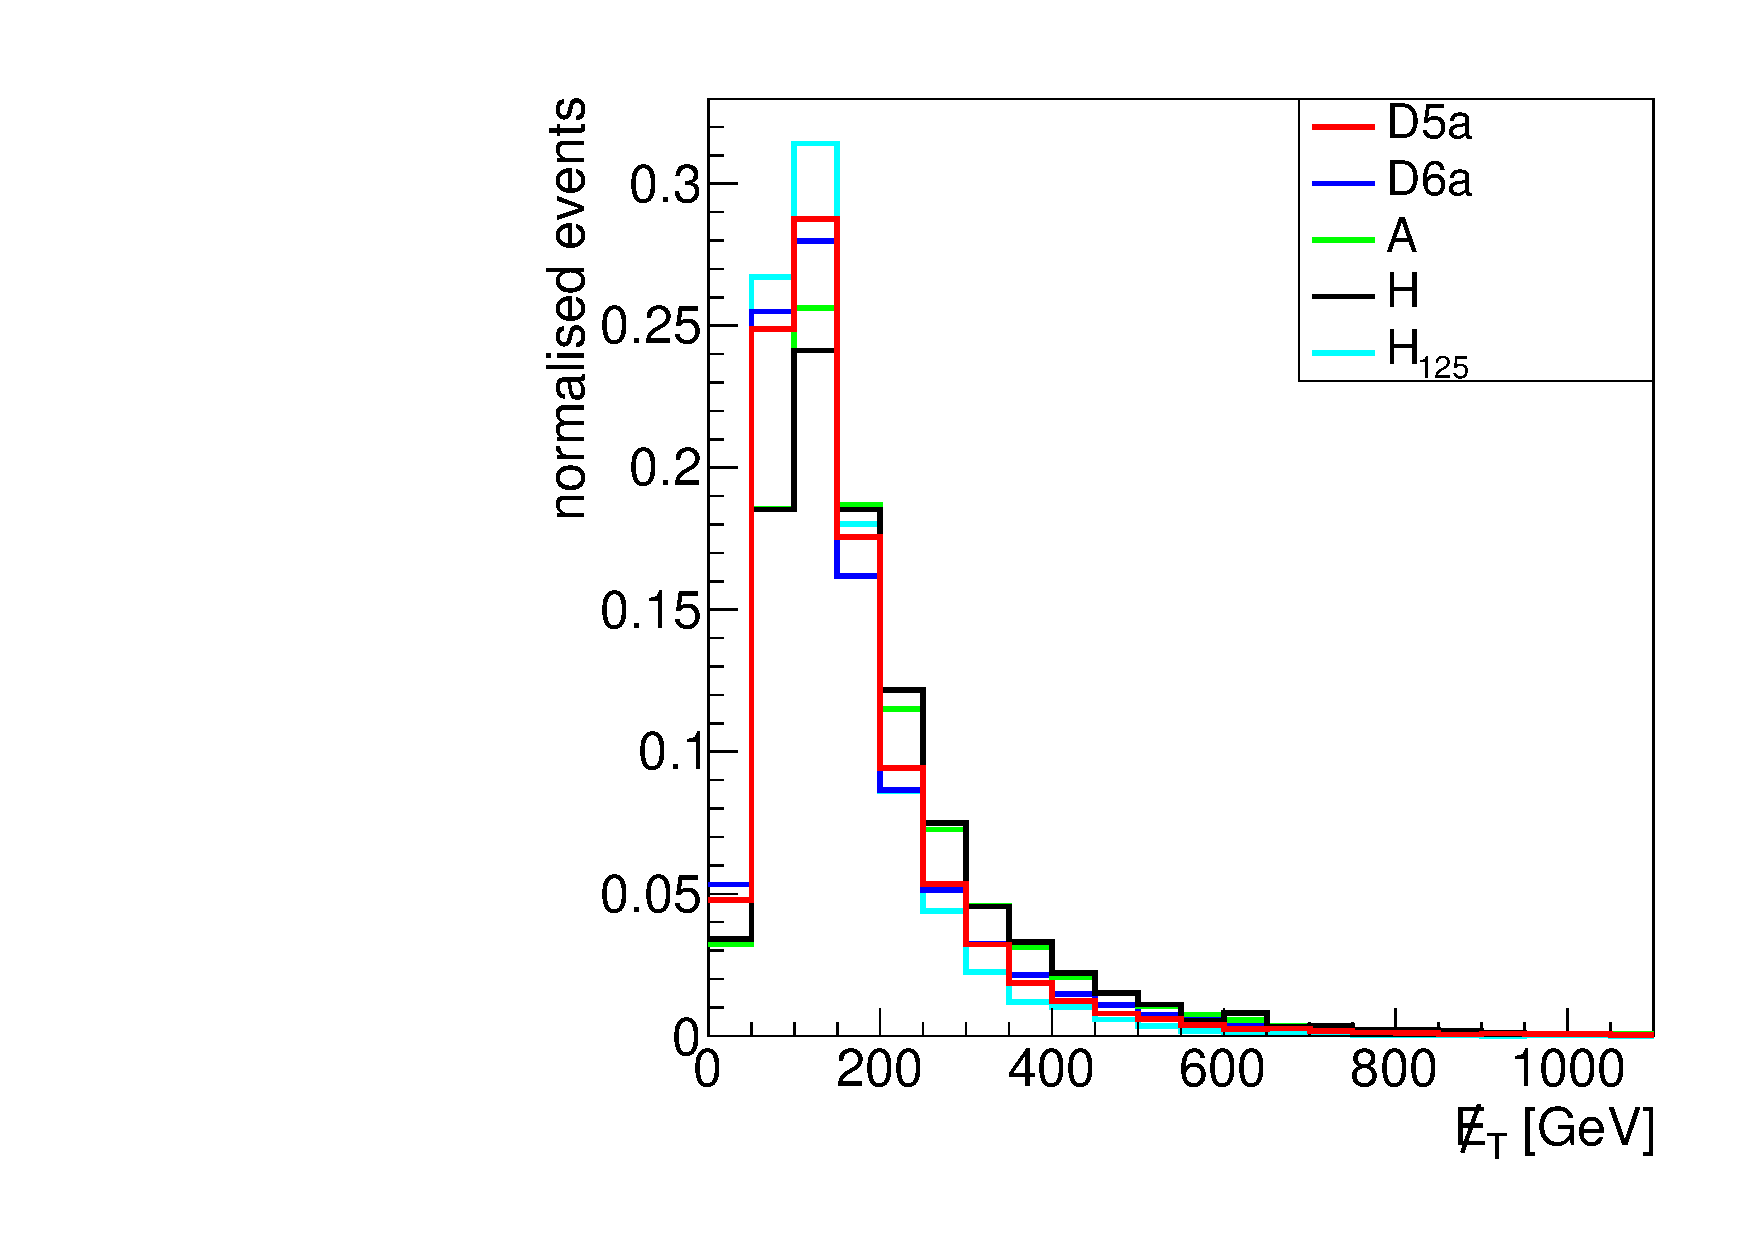
\includegraphics[width=.65\largefigwidth]{plots/interp/modelmet.pdf}}
  \subfloat[]{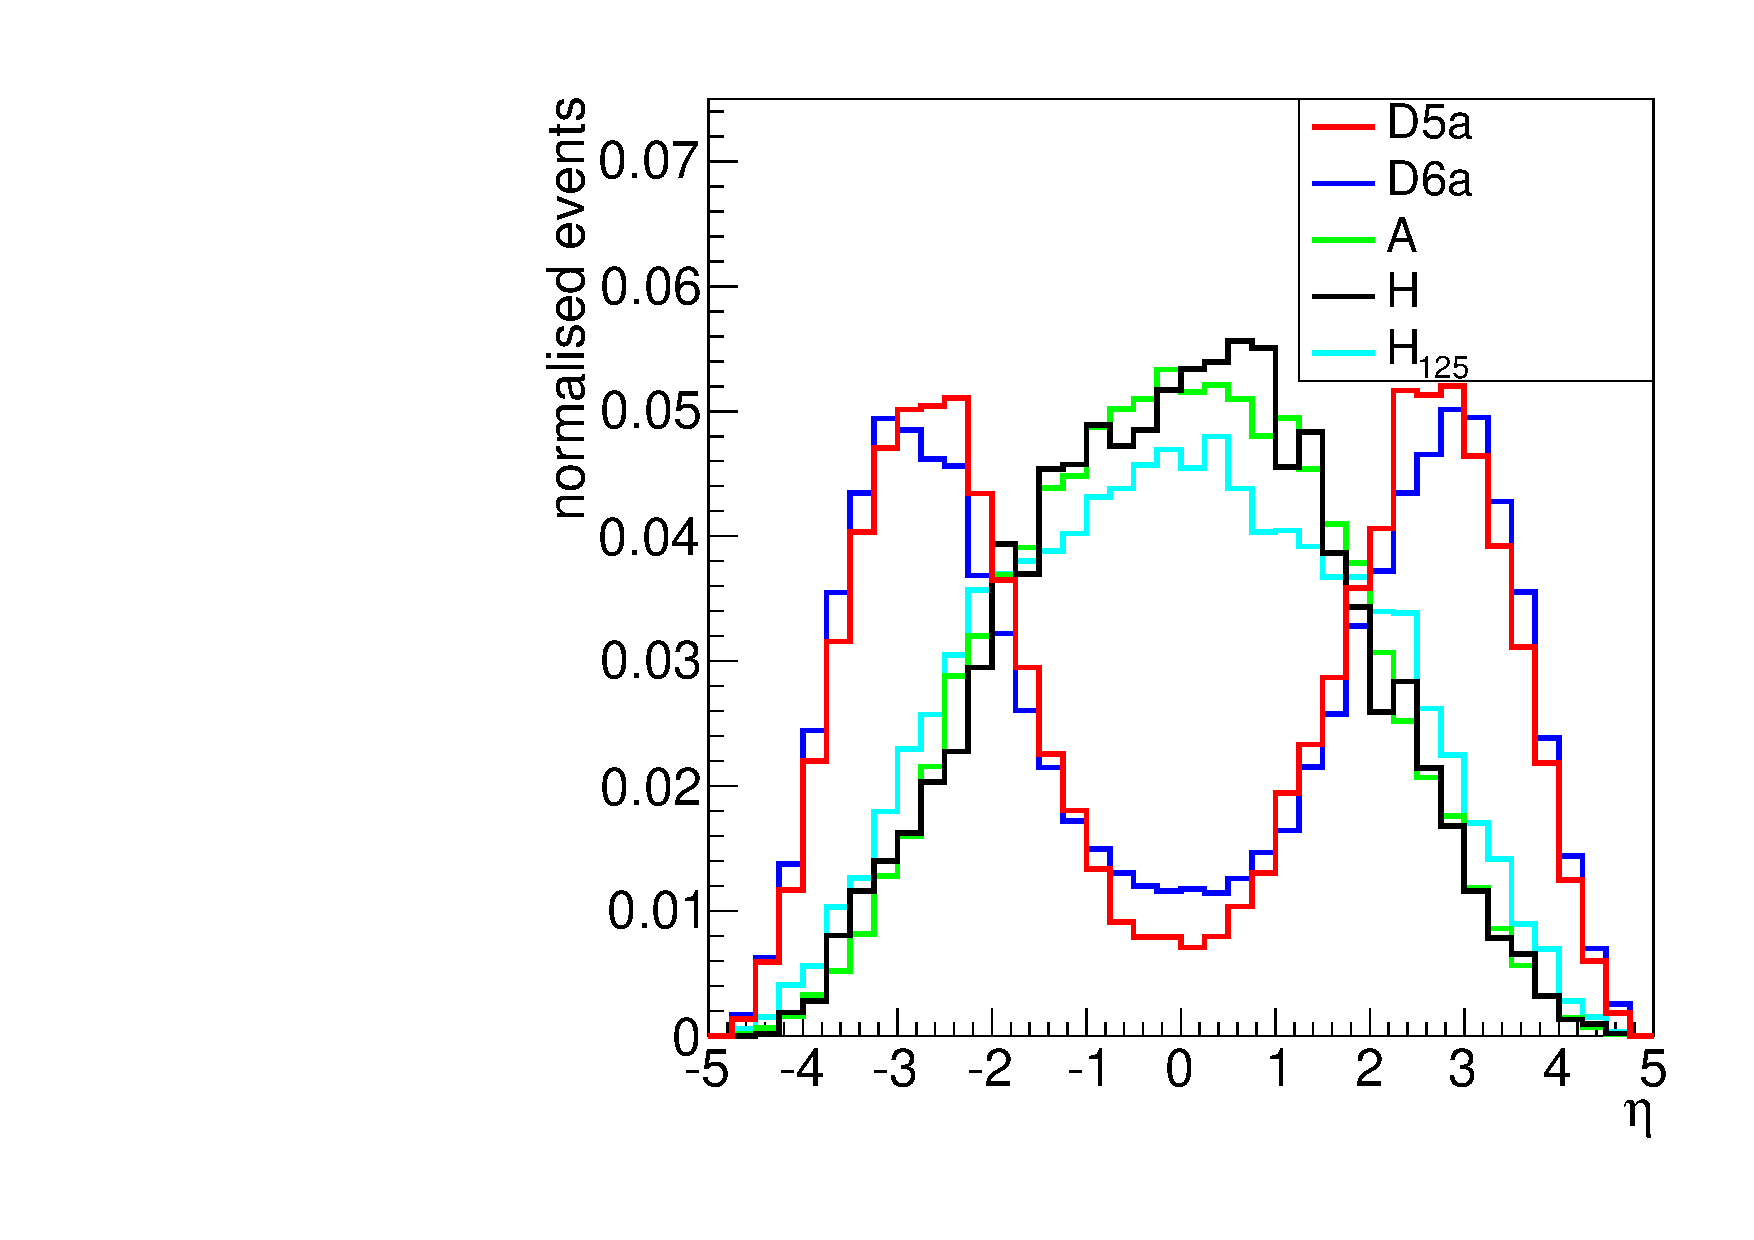
\includegraphics[width=.65\largefigwidth]{plots/interp/modeleta.pdf}}
  \caption{}%??
  \label{fig:dmmodelkinematics}
\end{figure}

\section{Results}
\label{sec:dmresults}
%??first project 125 GeV higgs limits on and off-shell
%??systematic scaling, both shown for on-shell just lumi scale from then on

\begin{figure}
  \subfloat[]{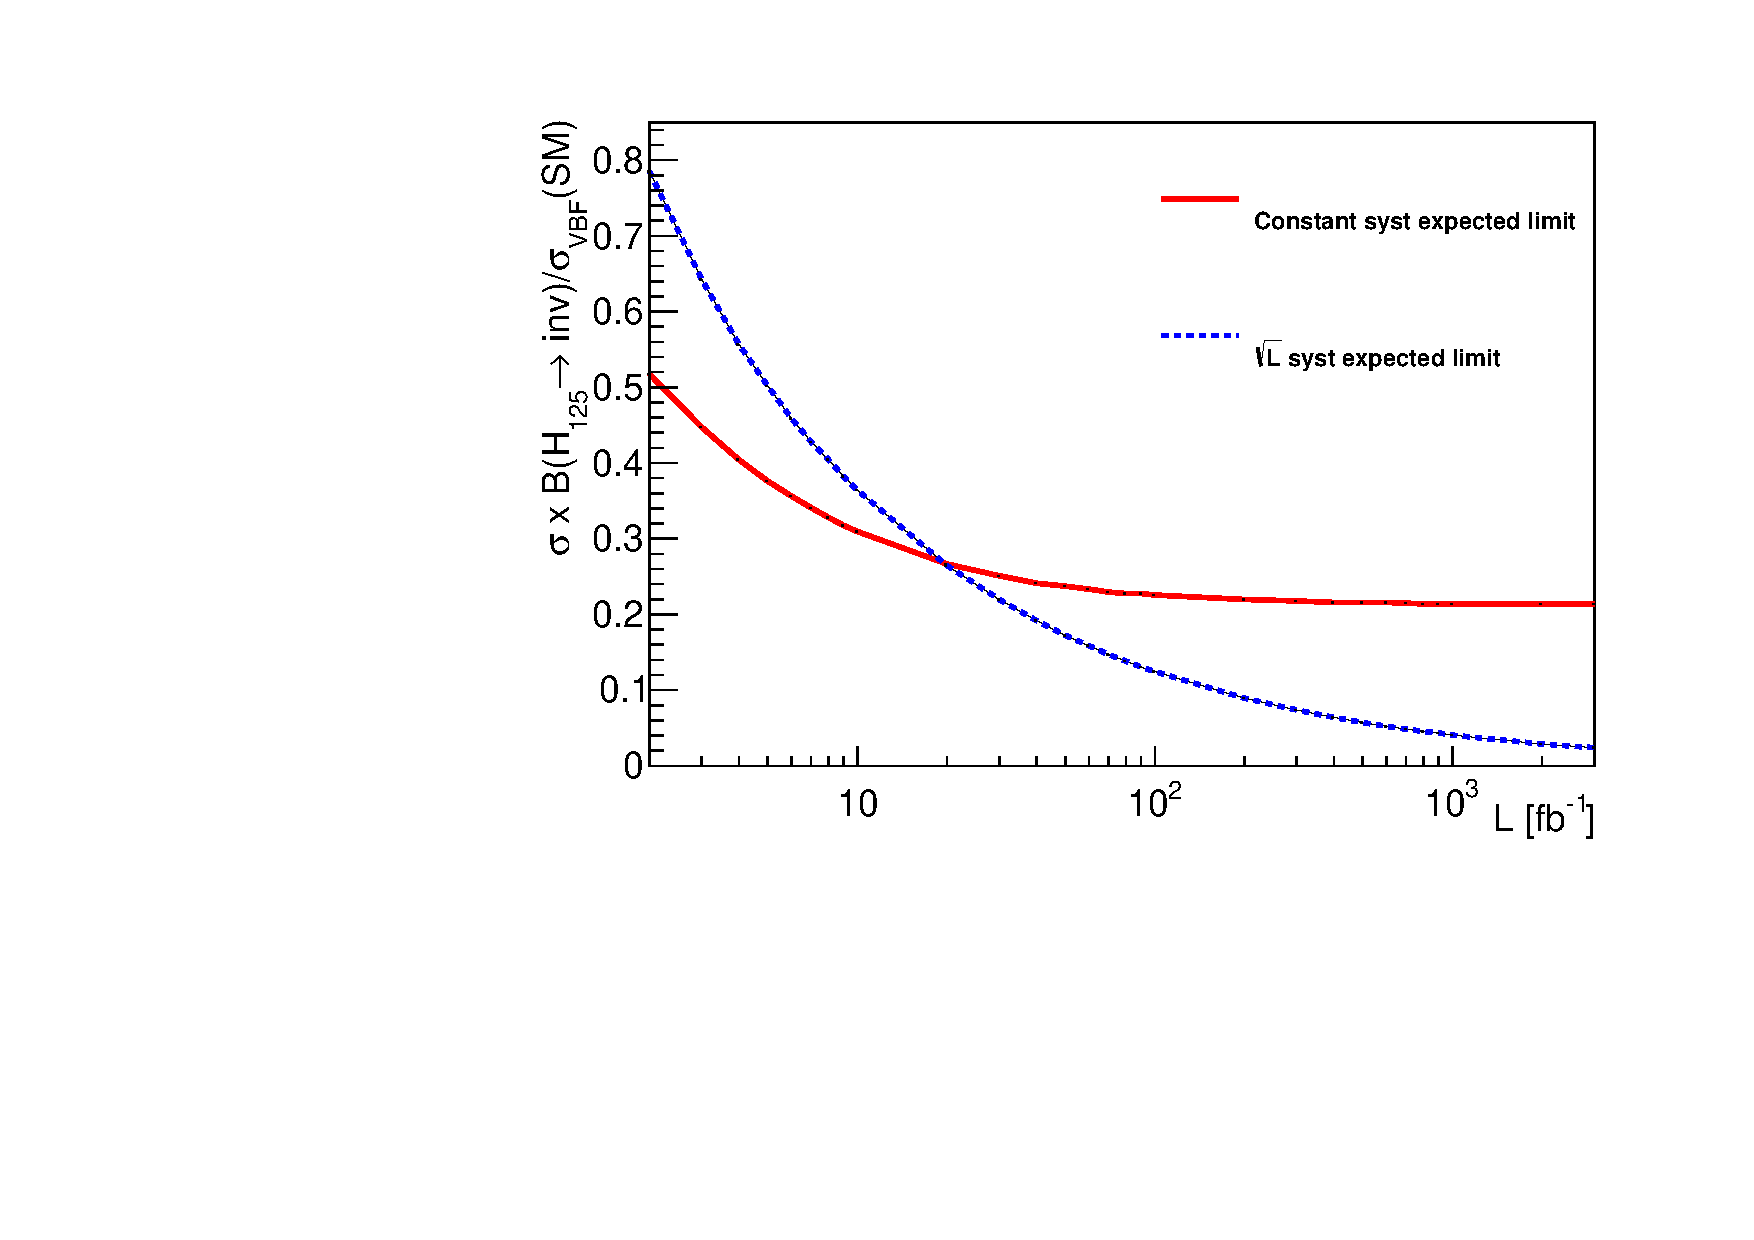
\includegraphics[width=\largefigwidth]{plots/interp/phenoprojectedvbflimit.pdf}}

  \subfloat[]{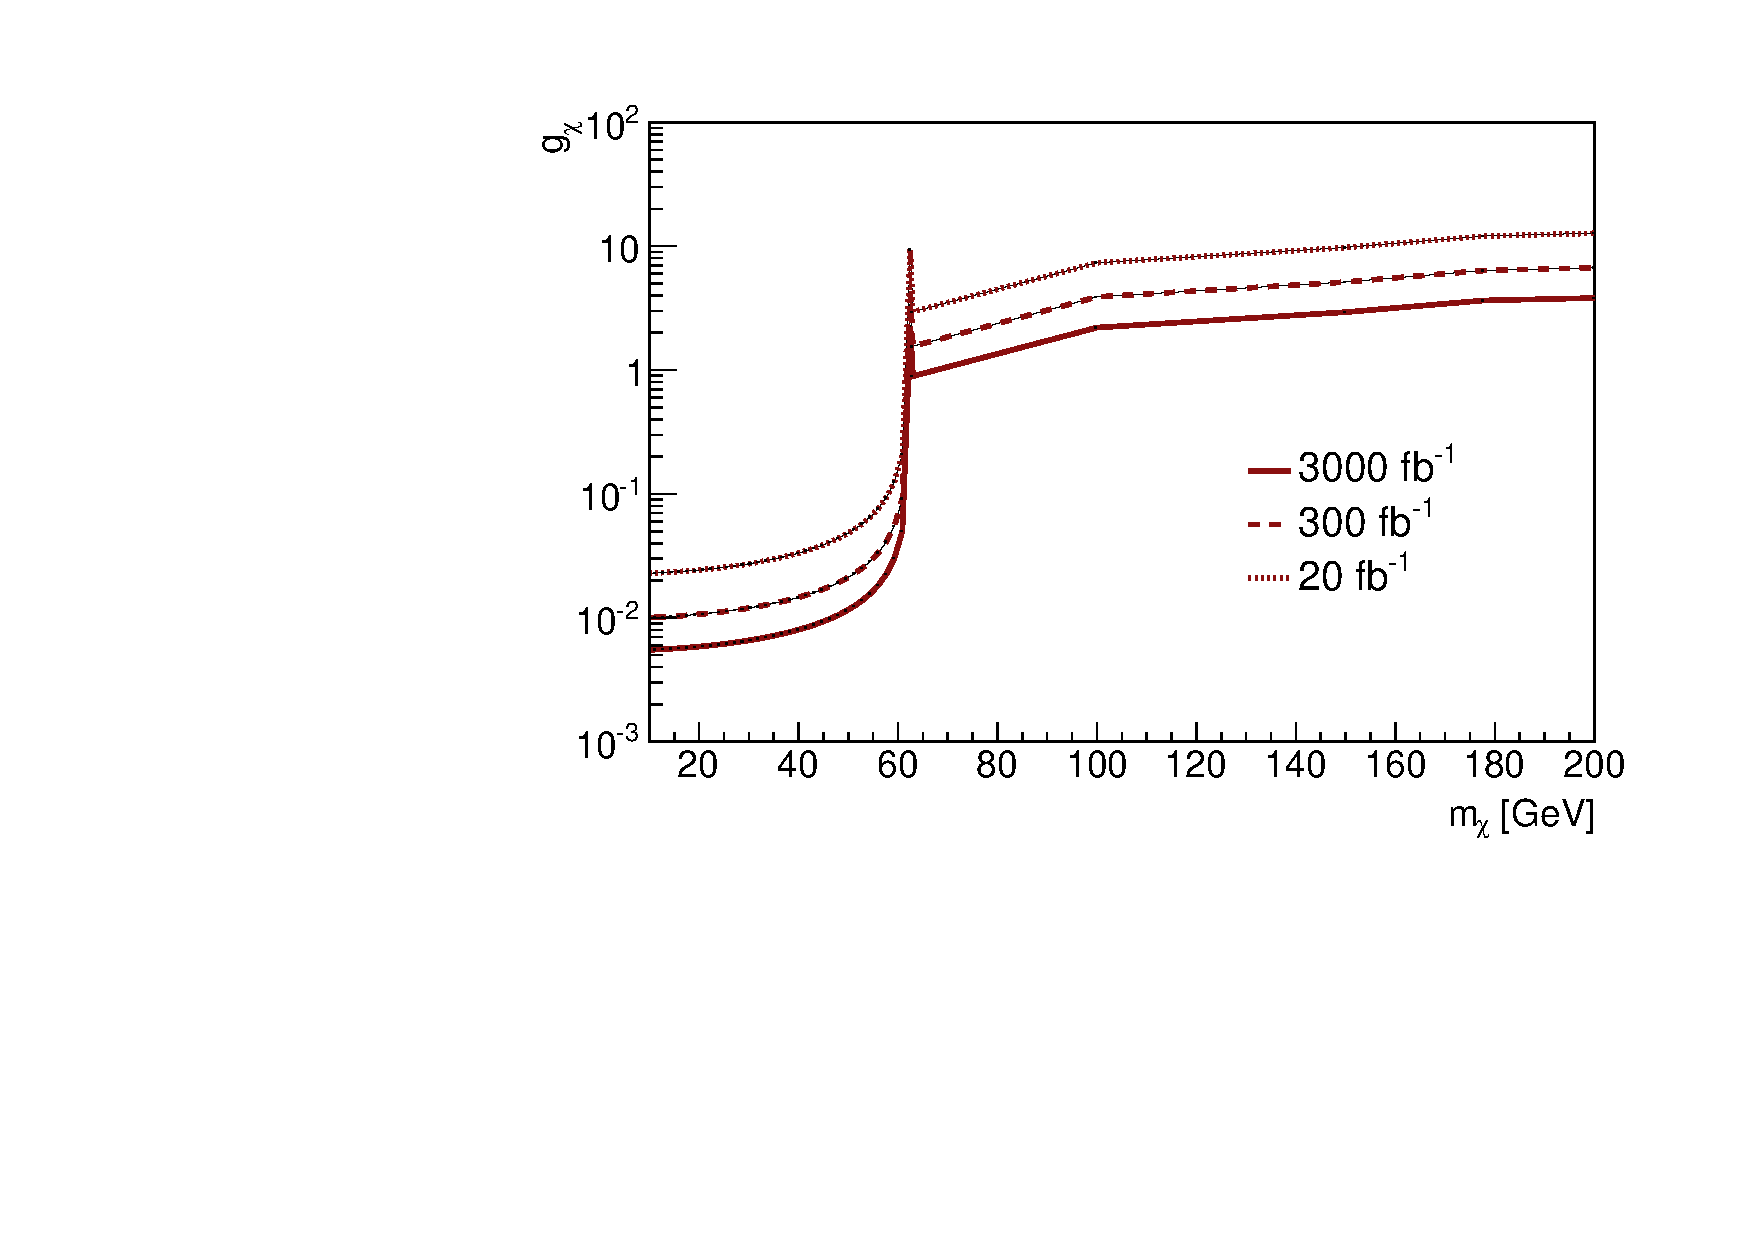
\includegraphics[width=\largefigwidth]{plots/interp/125higgsgchilimit.pdf}}
  \caption{}%??
  \label{fig:smprojectedlimits}
\end{figure}

%??non 125 GeV simplified models

\begin{figure}
  \subfloat[]{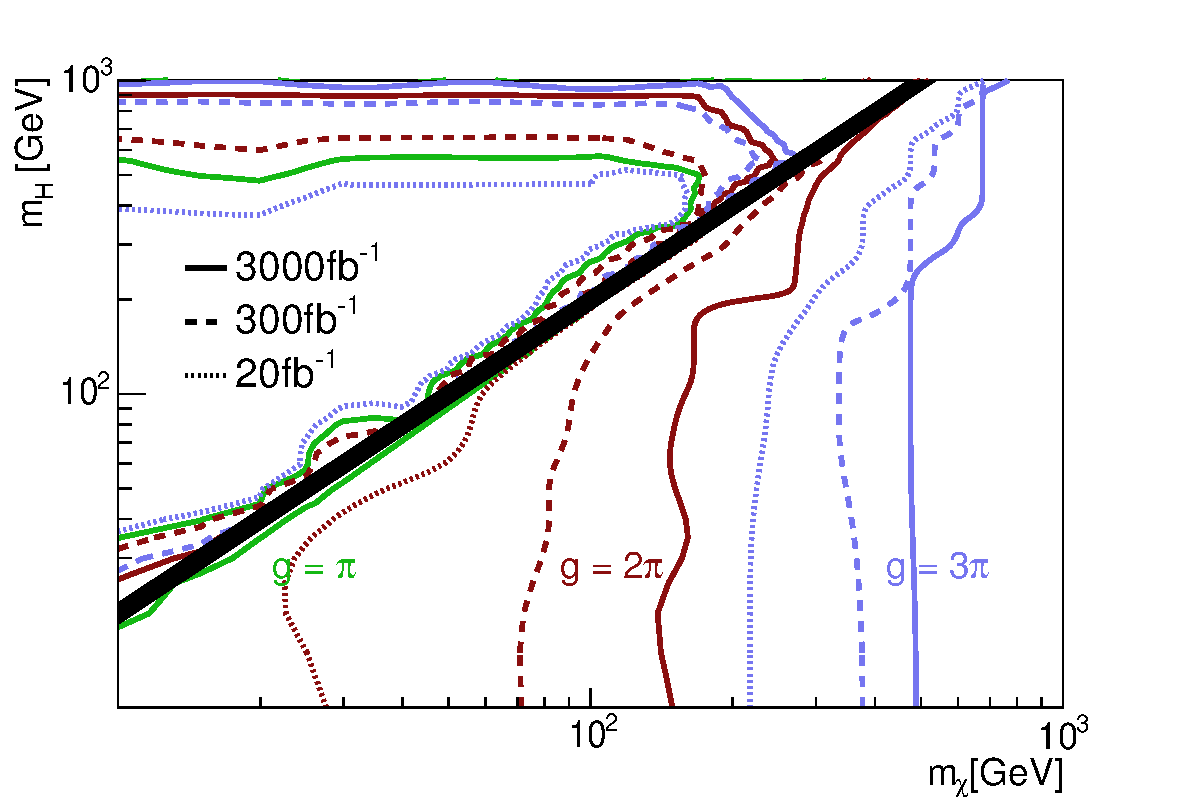
\includegraphics[width=\largefigwidth]{plots/interp/Hplane.pdf}}

  \subfloat[]{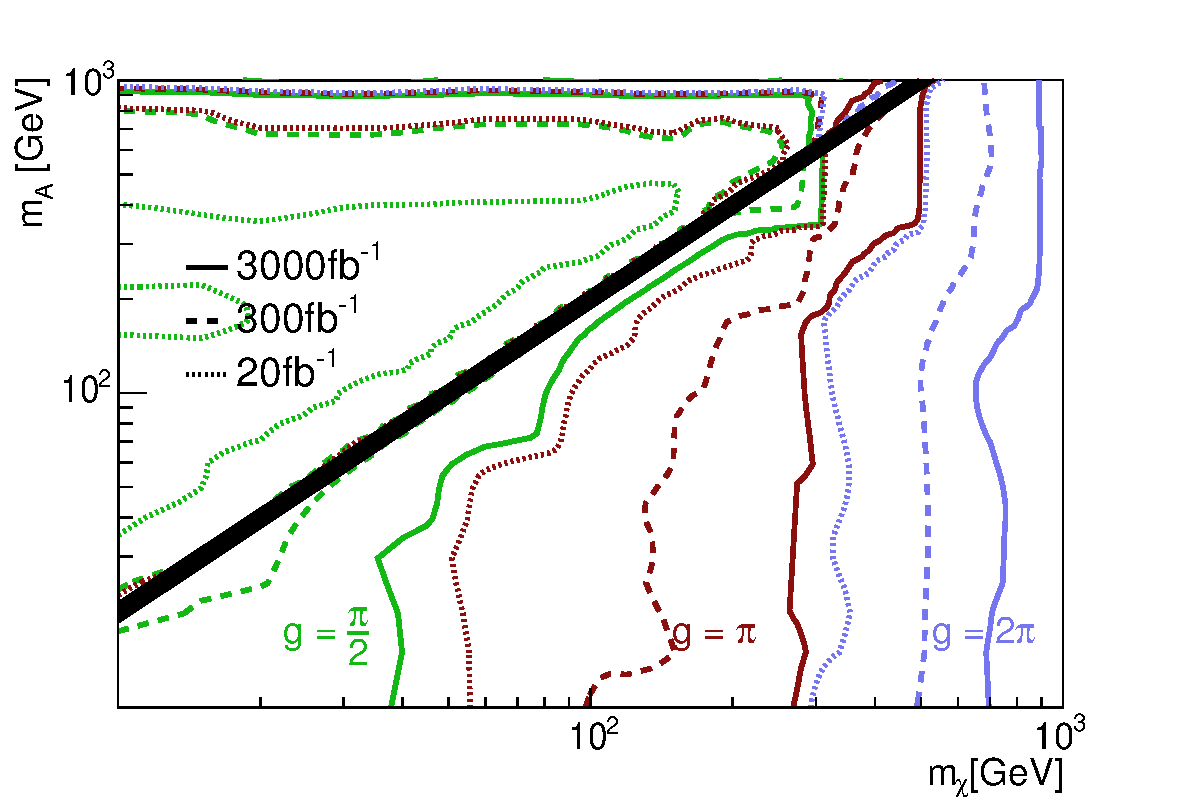
\includegraphics[width=\largefigwidth]{plots/interp/Aplane.pdf}}
  \caption{}%??
  \label{fig:simplifiedmodellimits}
\end{figure}

%??efts

\begin{figure}
  \subfloat[]{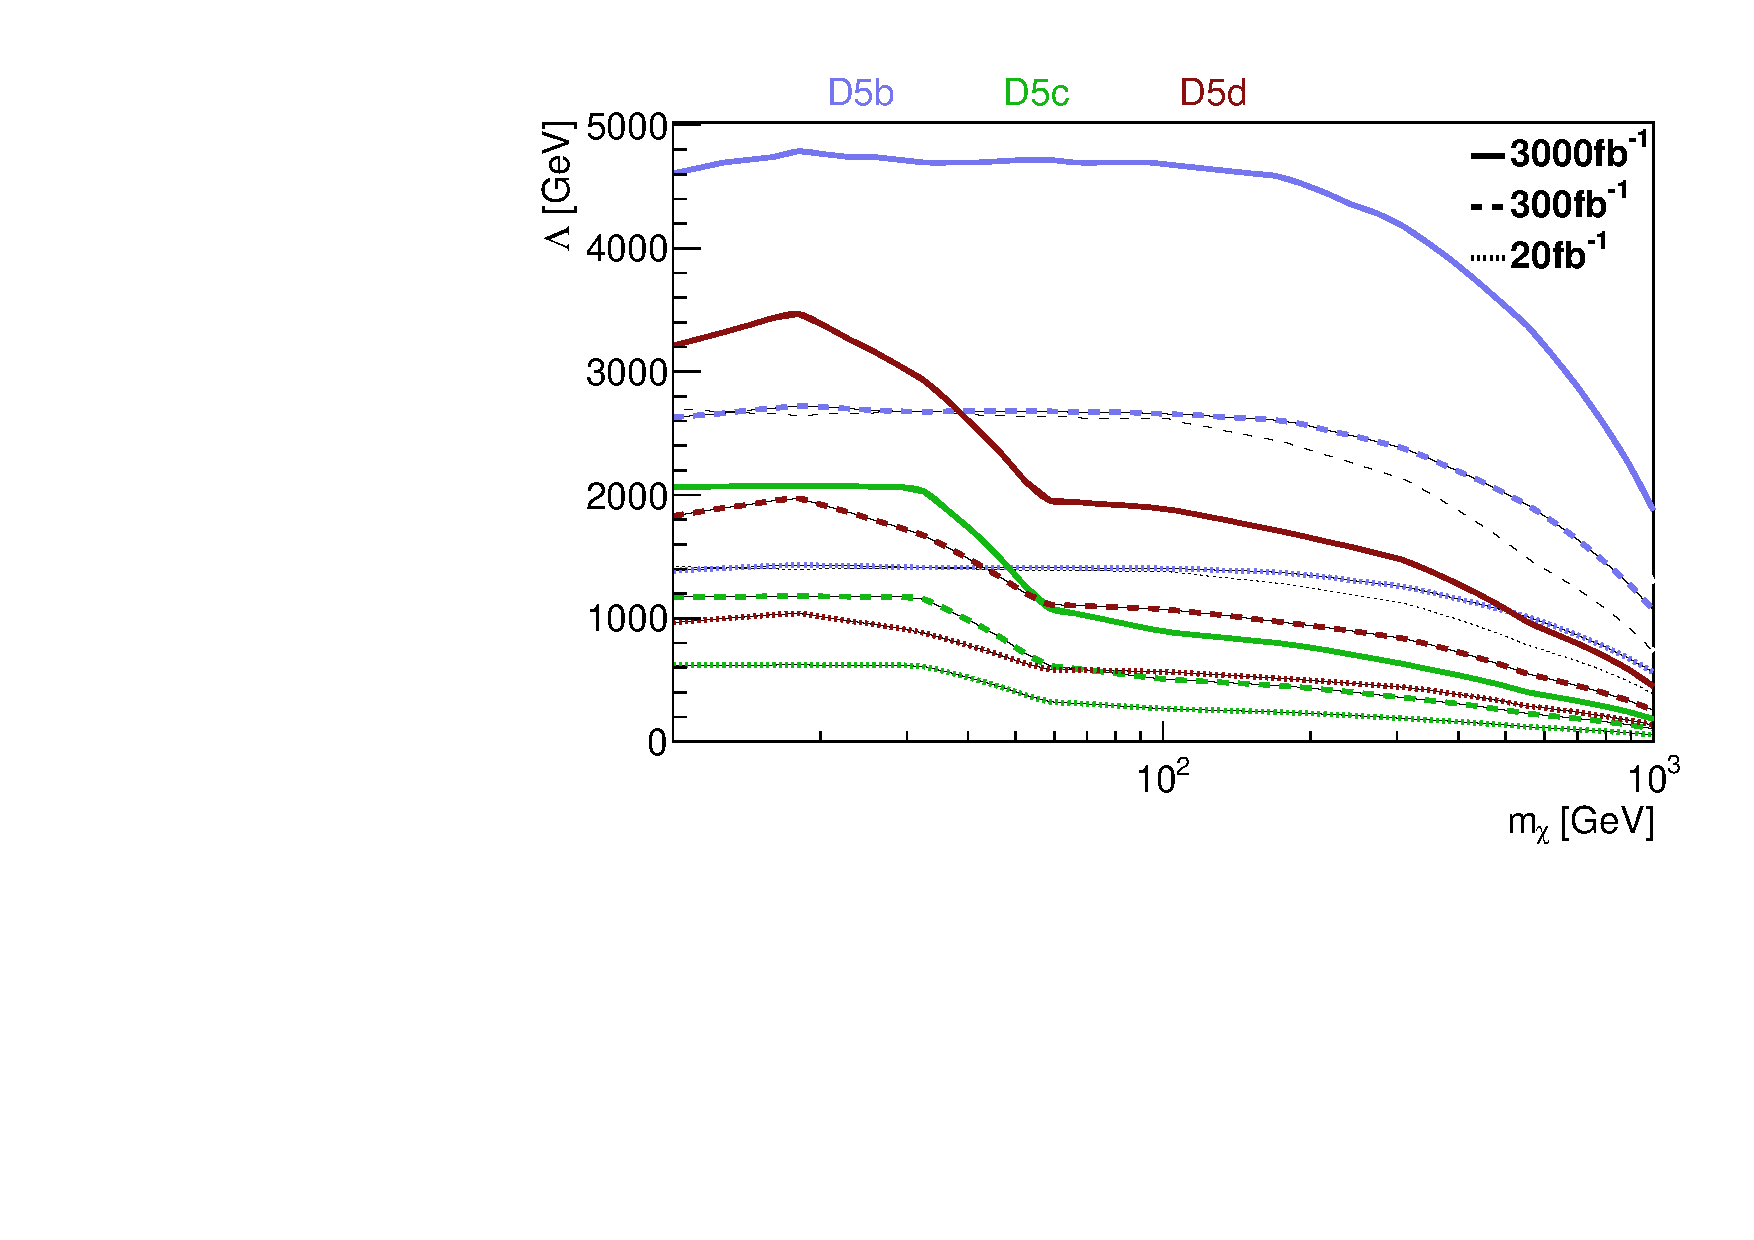
\includegraphics[width=.8\largefigwidth]{plots/interp/D5_multilumi.pdf}}

  \subfloat[]{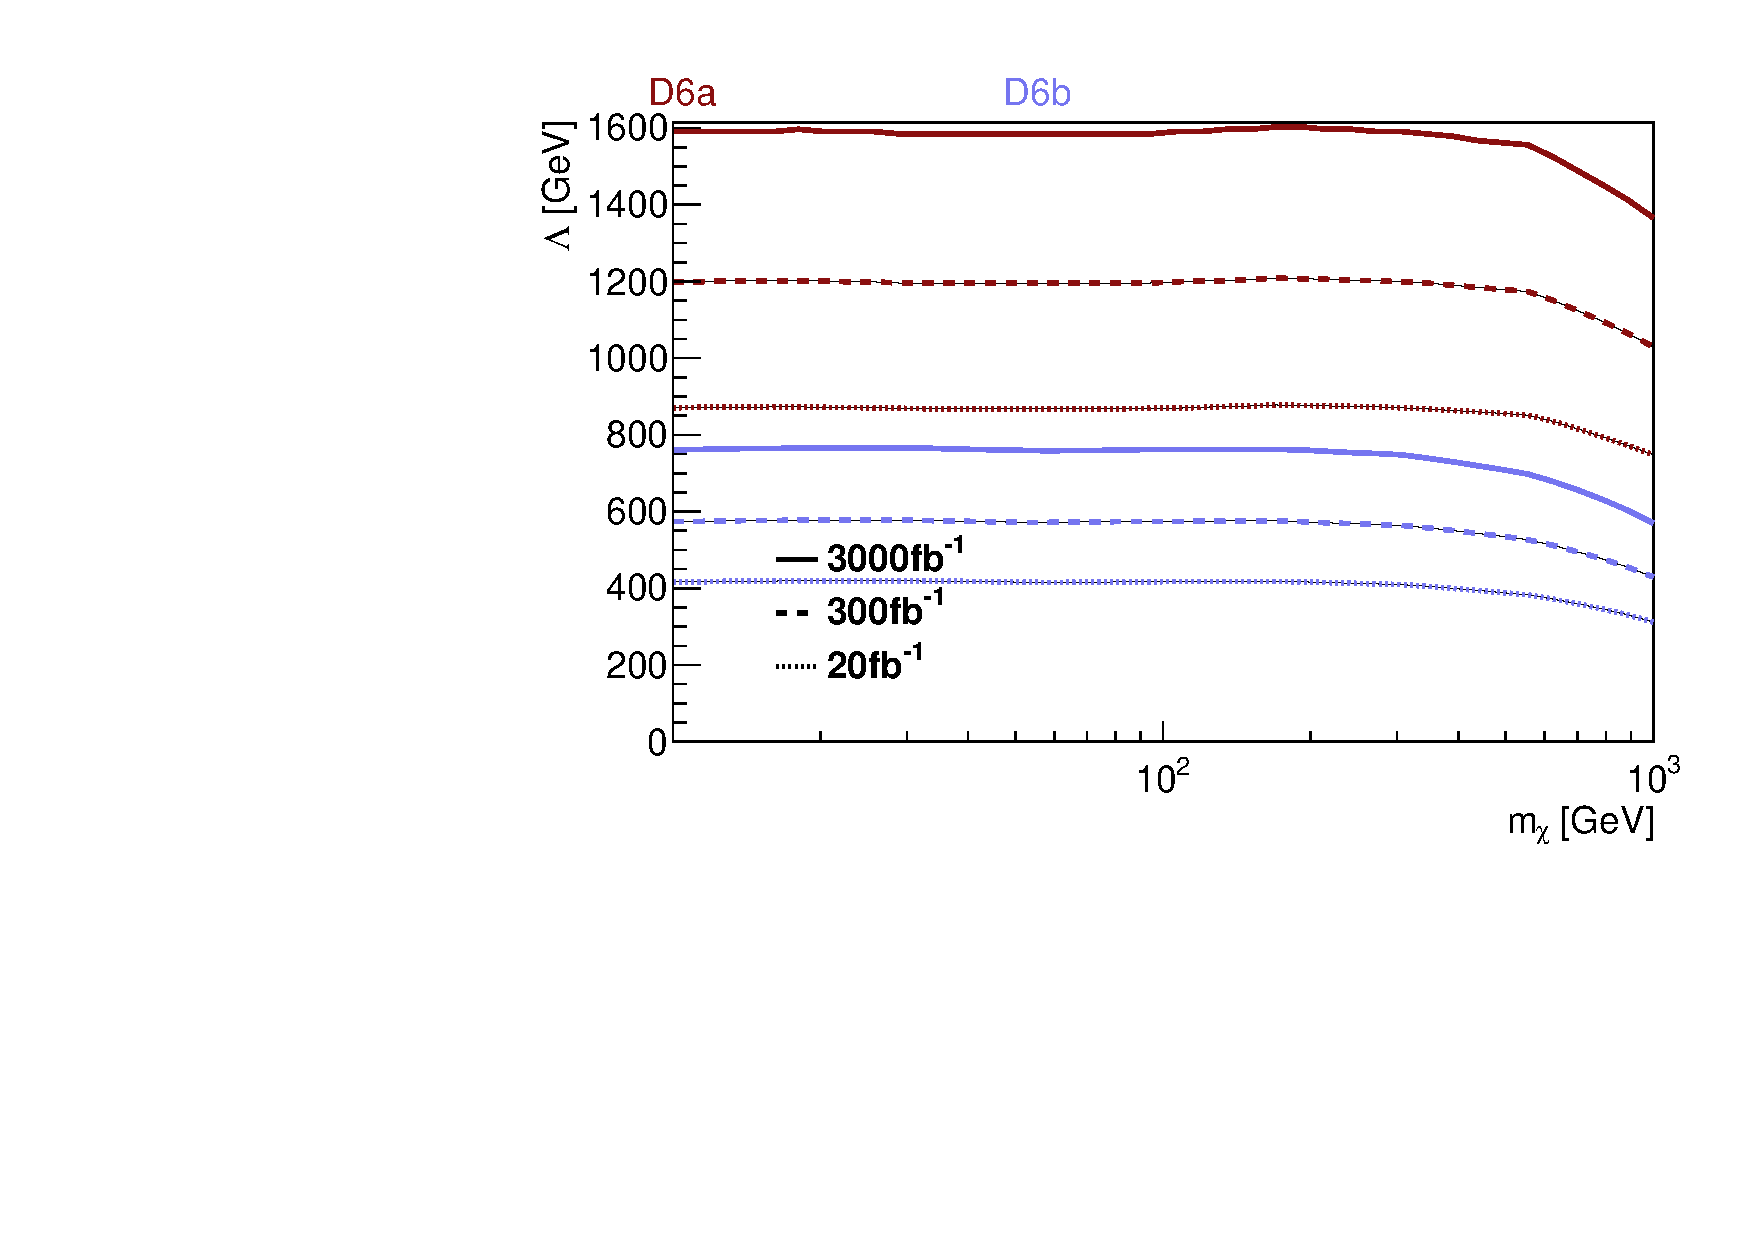
\includegraphics[width=.8\largefigwidth]{plots/interp/D6_2models.pdf}}

  \subfloat[]{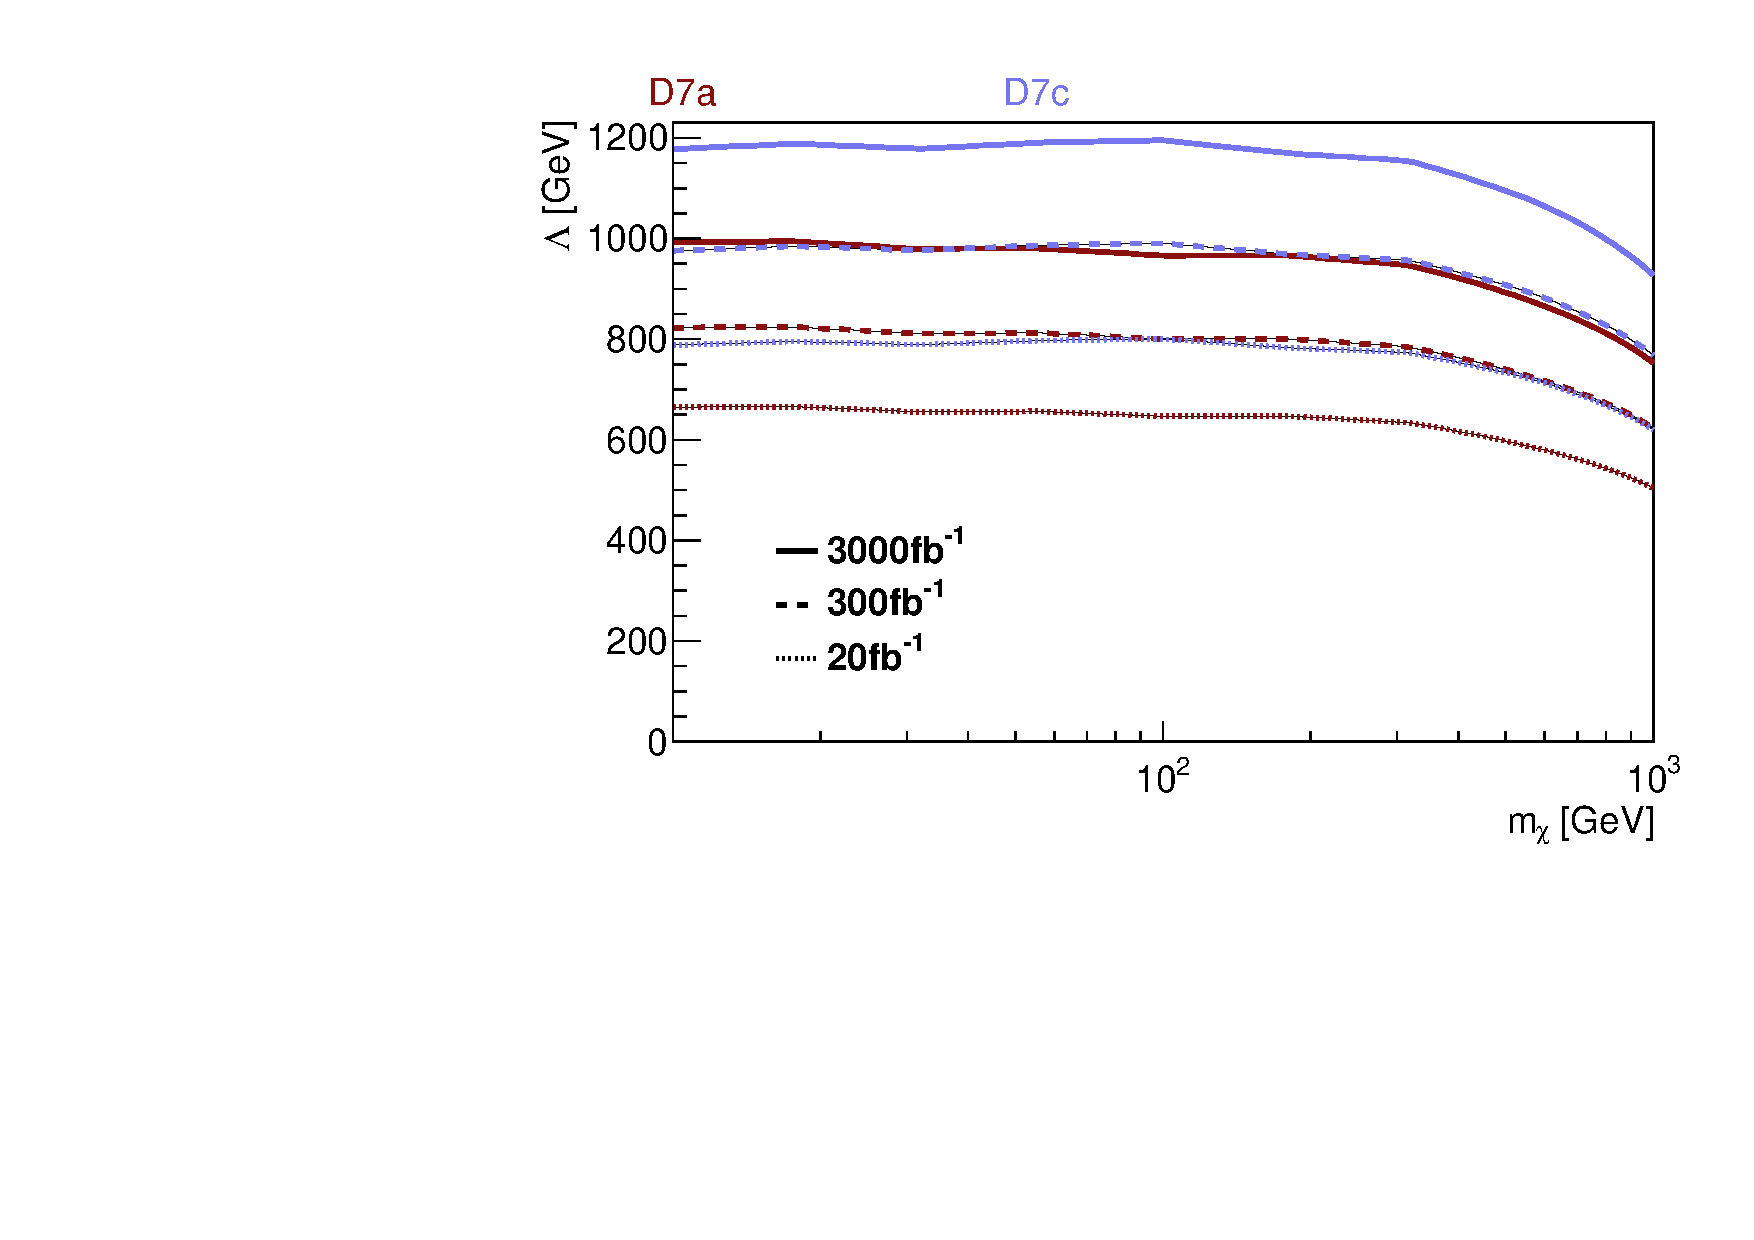
\includegraphics[width=.8\largefigwidth]{plots/interp/D7_2models.pdf}}
  \caption{}%??
  \label{fig:eftlimits}
\end{figure}

%??conclusion
